%!TEX program = xelatex
\documentclass[10pt]{beamer}
\usetheme{Darmstadt}
\usecolortheme{orchid}
\useinnertheme{rectangles}
\usepackage{eso-pic}
\usepackage{graphicx}
\usepackage{hyperref}
\usepackage{fontawesome5}
\usepackage{tabularx}
\usepackage{booktabs}
\usepackage{NWPU}


\begin{document}

% 封面页(带联系方式)
\begin{frame}[plain]
  \titlepage
\end{frame}

% 目录页
\begin{frame}[plain]{Outlines}
  \tableofcontents[hideallsubsections] %[hideallsubsections]隐藏subsection
\end{frame}
% ...existing code...

\section{Transformer Model Test Page}
\subsection{What is Transformer?}
\begin{frame}{Introduction to Transformer}
  \begin{block}{What is Transformer?}
    The Transformer is a deep learning model introduced in 2017\footnote{See Vaswani et al., 2017 for details.}, which relies entirely on attention mechanisms to draw global dependencies between input and output. It has become the foundation of most modern NLP models.
  \end{block}
  \begin{alertblock}{Why is it Important?}
    Transformers enable efficient parallel training and have revolutionized NLP, vision, and multimodal tasks.
  \end{alertblock}
  \begin{plainblock}{Fun Fact}
    The phrase "Attention is All You Need" comes from the original Transformer paper.
  \end{plainblock}
\end{frame}

\begin{frame}{Mathematical Formulation}
  \begin{block}{Scaled Dot-Product Attention}
    The core of Transformer is the attention mechanism, defined as:
    \[
      \text{Attention}(Q, K, V) = \text{softmax}\left(\frac{QK^\top}{\sqrt{d_k}}\right)V
    \]
    where $Q$ (queries), $K$ (keys), and $V$ (values) are projections of the input, and $d_k$ is the dimension of the keys.
  \end{block}
\end{frame}

\begin{frame}[fragile]{Python Example: Simple Transformer Block}
  \begin{block}{Code Example}
    \lstset{
      language=Python,
      basicstyle=\ttfamily\small,
      keywordstyle=\color{blue},
      commentstyle=\color{gray},
      stringstyle=\color{red},
      showstringspaces=false,
      breaklines=true,
      frame=single,
      backgroundcolor=\color{gray!10}
    }
    \begin{lstlisting}
import torch
import torch.nn as nn

class SimpleSelfAttention(nn.Module):
    def __init__(self, d_model):
        super().__init__()
        self.attn = nn.MultiheadAttention(d_model, num_heads=4)
    def forward(self, x):
        attn_output, _ = self.attn(x, x, x)
        return attn_output
# Example usage:
x = torch.rand(10, 32, 64)  # (seq_len, batch, d_model)
model = SimpleSelfAttention(64)
y = model(x)
    \end{lstlisting}
  \end{block}
\end{frame}

\begin{frame}{Transformer Architecture Diagram}
  \centering
  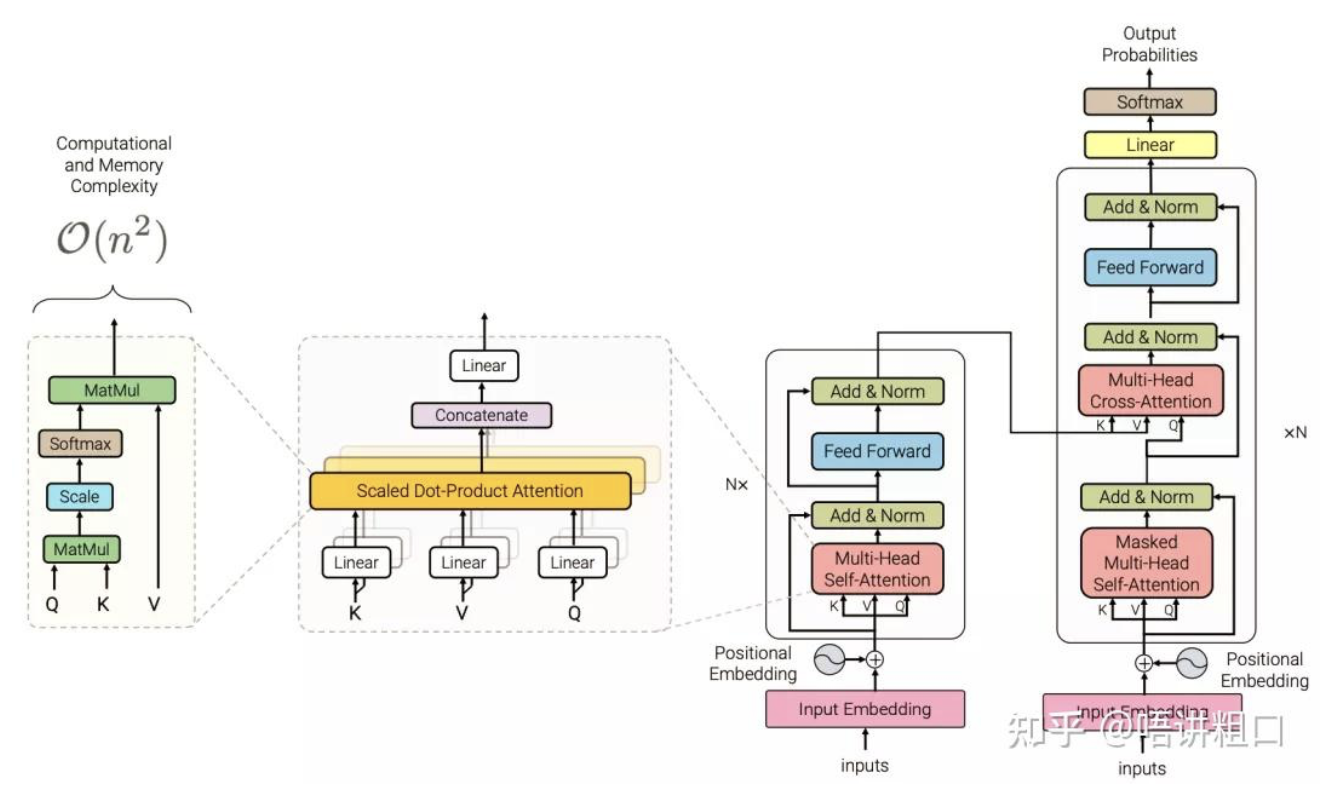
\includegraphics[width=0.7\textwidth]{illustration/image.png}
  \captionof{figure}{The architecture of the original Transformer model.}
\end{frame}

\begin{frame}{Comparison Table}
  \begin{block}{Transformer vs. RNN vs. CNN}
    \renewcommand{\arraystretch}{1.1}
    \begin{tabularx}{0.8\textwidth}{lccc}
      \toprule
      \footnotesize\textbf{Model} & \footnotesize\textbf{Parallel} & \footnotesize\textbf{Long-range} & \footnotesize\textbf{Application} \\
      \footnotesize & \footnotesize & \footnotesize\textbf{Dependency} & \footnotesize \\
      \midrule
      \footnotesize RNN & \footnotesize No & \footnotesize Weak & \footnotesize Sequence Modeling \\
      \footnotesize CNN & \footnotesize Partial & \footnotesize Limited & \footnotesize Vision, Sequence \\
      \footnotesize Transformer & \footnotesize Yes & \footnotesize Strong & \footnotesize NLP, Vision, Multimodal \\
      \bottomrule
    \end{tabularx}
  \end{block}
\end{frame}

% 参考文献页
\begin{frame}[allowframebreaks]{References}
  \footnotesize
  \begin{thebibliography}{99}
    \bibitem{vaswani2017attention}
      Vaswani, A., Shazeer, N., Parmar, N., et al.
      \newblock Attention is All You Need.
      \newblock In \emph{Advances in Neural Information Processing Systems}, 2017.
  \end{thebibliography}
\end{frame}



% 结语(带联系方式)
\section{The End}
\begin{frame}{Thank You!}
  \centering
  \Huge{\bfseries Any Questions?} 
  \vskip0.3cm
    \begin{tikzpicture}[inner sep=0,outer sep=0]
      \draw [black,line width=1.2pt,scope fading=fadetitleliner] (0,0) -- (\textwidth,0.0cm);
    \end{tikzpicture}%
    \vskip0.3cm
    \small
  \faEnvelope\ \url{xxxx@gmail.com} \quad

  \faGithub\ \url{github.com/xxxx} \quad

  \faPhone\ \url{(+86) 123-456-789} \\[1cm]
  \vfill
 \begin{tikzpicture}[remember picture,overlay]
    \node[anchor=south, xshift=0cm, yshift=0cm, opacity=0.25] at (current page.south) {
      
\includegraphics[width=\paperwidth]{logo/footbg.png} % 替换为你的图片路径
    };
  \end{tikzpicture}
\end{frame}

\end{document}